\begin{figure}[H]
    \centering
    \begin{subfigure}{.38\textwidth}
        \centering
        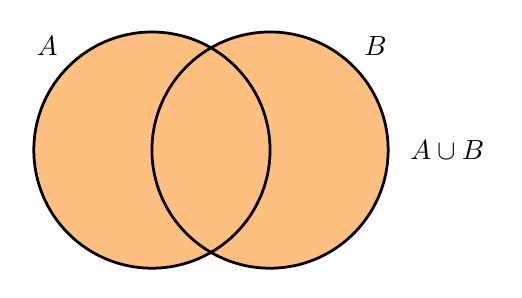
\begin{tikzpicture}[scale=1.5]
            \draw[fill=orange!50] (0,0) circle(1);
            \draw[fill=orange!50] (1,0) circle(1);
            \node[draw, circle, line width=1pt, minimum size=3cm, label={135:$A$}] at (0,0) {};
            \node[draw, circle, line width=1pt, minimum size=3cm, label={45:$B$}] at (1,0) {};
            \node at (2.5,0) {$A \cup B$};
        \end{tikzpicture}
    \end{subfigure}
    \begin{subfigure}{.38\textwidth}
        \centering
        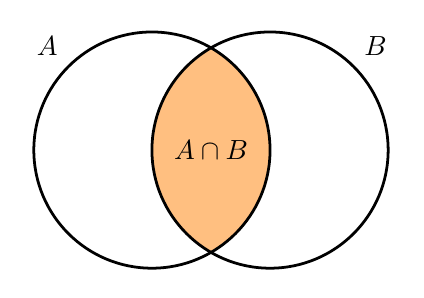
\begin{tikzpicture}[scale=1.5]
            \begin{scope}
                \clip (0,0) circle(1cm);
                \clip (1,0) circle(1cm);
                \fill[orange!50] (0,0) circle(1cm);
            \end{scope}
            \node[draw, circle, line width=1pt, minimum size=3cm, label={135:$A$}] at (0,0) {};
            \node[draw, circle, line width=1pt, minimum size=3cm, label={45:$B$}] at (1,0) {};
            \node at (0.5,0) {$A \cap B$};
        \end{tikzpicture}
    \end{subfigure}
\end{figure}